\documentclass[10pt]{beamer}

\usetheme[progressbar=frametitle]{metropolis}
\usepackage{appendixnumberbeamer}

\usepackage{booktabs}
\usepackage[scale=2]{ccicons}

\usepackage{tcolorbox}
\definecolor{darkred}{RGB}{173,34,48}

\usepackage{pgfplots}
\usepgfplotslibrary{dateplot}
\usepackage{tikz}
\usepackage{xeCJK} %导入中文包
\setCJKmainfont{SimHei} %中文字体采用黑体  Microsoft YaHei

%\usepackage{pgfplots}
%\usepgfplotslibrary{dateplot}
%\usepackage{tikz}
\usetikzlibrary{shapes.geometric}
%\usetikzlibrary{decorations.markings}
\usetikzlibrary{calc,decorations.markings}
\usepackage{xspace}
\newcommand{\themename}{\textbf{\textsc{metropolis}}\xspace}
\usepackage{xcolor}
	\definecolor{limegreen}{rgb}{0.2, 0.8, 0.2}
\definecolor{nicegreen}{RGB}{102,252,102}
\definecolor{mediumturquoise}{rgb}{0.28, 0.82, 0.8}
\definecolor{oceanboatblue}{rgb}{0.0, 0.47, 0.75}
\definecolor{darkred}{rgb}{0.675,0,0.2}

\newcommand{\dif}{\mathrm{d}}
\newcommand{\me}{\mathrm{e}}
%\newcommand{\mi}{\mathrm{i}}


%================================================================================================================
\newcommand{\fwbox}[2]{\text{\makebox[#1][c]{$\hspace{-150pt}\displaystyle#2\hspace{-150pt}$}}}
\newcommand{\fwboxL}[2]{\text{\makebox[#1][l]{$#2$}}}
\newcommand{\fwboxR}[2]{\text{\makebox[#1][r]{$#2$}}}
\newcommand{\bigger}[1]{\raisebox{-0.95pt}{\scalebox{1.25}{$#1$}}}
\newcommand{\Bigger}[1]{\raisebox{-2.25pt}{\scalebox{1.75}{$#1$}}}
\renewcommand{\Bar}{\overline}
\renewcommand{\tilde}{\widetilde}
\newcommand{\eq}[1]{\vspace{-0.5pt}\begin{equation}\hspace{0pt}#1\hspace{-0pt}\vspace{-0.5pt}\end{equation}}
\newcommand{\fig}[2]{\vcenter{\includegraphics[scale=#1]{#2}}}
\newcommand{\mi}{\raisebox{0.75pt}{\scalebox{0.75}{$\hspace{-1pt}\,-\,\hspace{-0.75pt}$}}}
\newcommand{\pl}{\raisebox{0.75pt}{\scalebox{0.75}{$\hspace{-1pt}\,+\,\hspace{-0.75pt}$}}}
\newcommand{\ab}[1]{\langle #1\rangle}
\newcommand{\equivR}{\fwbox{14.5pt}{\hspace{-0pt}\fwboxR{0pt}{\raisebox{0.47pt}{\hspace{1.25pt}:\hspace{-4pt}}}=\fwboxL{0pt}{}}}
\newcommand{\equivL}{\fwbox{14.5pt}{\fwboxR{0pt}{}=\fwboxL{0pt}{\raisebox{0.47pt}{\hspace{-4pt}:\hspace{1.25pt}}}}}
\renewcommand{\u}[2]{(\hspace{-0.5pt}#1;\hspace{-1.5pt}#2\hspace{-0.5pt})}
\newcommand{\proj}[1]{\raisebox{1.75pt}{\big[}\hspace{-0.75pt}#1\hspace{-0.75pt}\raisebox{1.75pt}{\big]}}
\renewcommand{\r}[1]{\mathfrak{A}\hspace{-0.75pt}(\hspace{-1pt}{\color{hred}#1\hspace{-1pt}})}
\newcommand{\rb}[2]{(\hspace{-1pt}{\color{hblue}#1}\hspace{-1pt})^c_{\fwboxL{4.5pt}{#2}}}
\newcommand{\amp}[1]{\mathfrak{A}_{{\color{hred}#1}}}
\newcommand{\f}[1]{\mathfrak{#1}}
\newcommand{\Zeta}[1]{\zeta_#1}
\newcommand{\Li}[2]{\hspace{1pt}\mathrm{Li}_{#1}(#2)}

\newcommand{\polyalpha}{\rho}
\newcommand{\polybeta}{\sigma}


\definecolor{hblue}{rgb}{0,0,0.575}
\definecolor{hred}{rgb}{0.575,0.0,0.225}
\definecolor{hteal}{rgb}{0.0,0.545,0.7451}
\definecolor{optLegColour}{rgb}{0.5,0.5,0.5}



\def\figScale{0.835}\def\edgeLen{1*\figScale}\def\fScale{\small}\def\legLen{\edgeLen*0.65}\def\labelDist{\legLen*1.45}\def\lineThickness{(1pt)}\def\dotSize{(\figScale*10)}\def\ampSize{(1*\figScale*10pt)}\def\legSpread{5}\def\extLegLen{0.75*0.75*\figScale}
\tikzset{ddot/.style={fill=black,circle,minimum size=0.35*\dotSize,inner sep=0}}
\tikzset{int/.style={black,line width=\lineThickness,line cap=round,rounded corners=0.5pt}}\tikzset{ext/.style={black,line width=\lineThickness,line cap=round}}\tikzset{bdot/.style={fill=black,circle,minimum size=0.45*\ampSize,inner sep=0}}\tikzset{wdot/.style={draw=black,line width=\lineThickness,fill=white,circle,minimum size=0.65*\ampSize,inner sep=0}}
\newcommand{\leg}[3]{\draw[ext] #1--($#1+(#2:\legLen)$);\node at ($#1+(#2:\labelDist)$)[]{{\fScale #3}};}
\newcommand{\optLeg}[2]{\coordinate (aa0) at #1;\coordinate (aa5) at ($#1+(#2+\legSpread*3:\extLegLen)$);\coordinate (bb5) at ($#1+(#2-\legSpread*3:\extLegLen)$);\coordinate (aa1) at ($(aa0)!0.4!(aa5)$);\coordinate (aa2) at ($(aa0)!0.55!(aa5)$);\coordinate (aa3) at ($(aa0)!0.7!(aa5)$);\coordinate (aa4) at ($(aa0)!0.85!(aa5)$);\coordinate (bb1) at ($(aa0)!0.4!(bb5)$);\coordinate (bb2) at ($(aa0)!0.55!(bb5)$);\coordinate (bb3) at ($(aa0)!0.7!(bb5)$);\coordinate (bb4) at ($(aa0)!0.85!(bb5)$);\fill[optLegColour] (aa0)--(aa1)--(bb1)--(aa0);\fill[optLegColour] (aa2)--(aa3)--(bb3)--(bb2)--(aa2);\fill[optLegColour] (aa4)--(aa5)--(bb5)--(bb4)--(aa4);}

\newcommand{\octagonk}{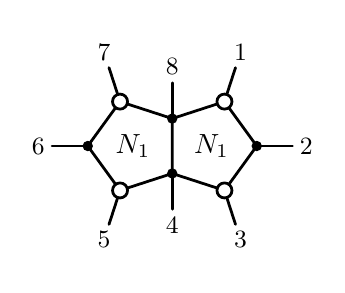
\begin{tikzpicture}[scale=\figScale,baseline=-2.45]\useasboundingbox ($(-7.9/3*\figScale,-1.8)$) rectangle ($(7.9/3*\figScale,1.8)$);\draw[int,line width=0.1,red,draw=none] ($(-7.5/3*\figScale,-1.5)$) rectangle ($(7.5/3*\figScale,1.5)$);\coordinate(v1) at ($(0,0)+(90:\edgeLen/2)$);\coordinate(v2)at($(v1)+(18:\edgeLen)$);\coordinate(v3)at($(v2)+(18-72:\edgeLen)$);\coordinate(v4)at($(v3)+(18-2*72:\edgeLen)$);\coordinate(v5)at($(v4)+(18-3*72:\edgeLen)$);\coordinate(v6)at($(v5)+(198-0*72:\edgeLen)$);\coordinate(v7)at($(v6)+(198-1*72:\edgeLen)$);\coordinate(v8)at($(v7)+(198-2*72:\edgeLen)$);
\draw[int](v1)--(v2)--(v3)--(v4)--(v5)--(v6)--(v7)--(v8)--(v1);\draw[int](v1)--(v5);\leg{(v1)}{90}{8};\leg{(v2)}{72}{1};\leg{(v3)}{72-1*72}{\!2};\leg{(v4)}{72-2*72}{3};\leg{(v5)}{-90}{4};\leg{(v6)}{252-0*72}{5};\leg{(v7)}{252-1*72}{6\!};\leg{(v8)}{252-2*72}{7};\foreach\a in {1,3,5,7}{\node at (v\a) [bdot]{};};\foreach\a in {2,4,6,8}{\node at (v\a) [wdot]{};};
\node at ($(\edgeLen/1.4,0)$) []{$N_1$};\node at ($(-\edgeLen/1.4,0)$) []{$N_1$};
\end{tikzpicture}}
\newcommand{\octagonkPrime}{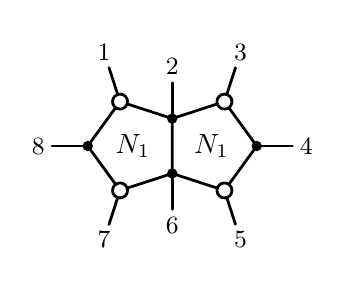
\begin{tikzpicture}[scale=\figScale,baseline=-2.45]\useasboundingbox ($(-7.9/3*\figScale,-1.8)$) rectangle ($(7.9/3*\figScale,1.8)$);\draw[int,line width=0.1,red,draw=none] ($(-7.5/3*\figScale,-1.5)$) rectangle ($(7.5/3*\figScale,1.5)$);\coordinate(v1) at ($(0,0)+(90:\edgeLen/2)$);\coordinate(v2)at($(v1)+(18:\edgeLen)$);\coordinate(v3)at($(v2)+(18-72:\edgeLen)$);\coordinate(v4)at($(v3)+(18-2*72:\edgeLen)$);\coordinate(v5)at($(v4)+(18-3*72:\edgeLen)$);\coordinate(v6)at($(v5)+(198-0*72:\edgeLen)$);\coordinate(v7)at($(v6)+(198-1*72:\edgeLen)$);\coordinate(v8)at($(v7)+(198-2*72:\edgeLen)$);
\draw[int](v1)--(v2)--(v3)--(v4)--(v5)--(v6)--(v7)--(v8)--(v1);\draw[int](v1)--(v5);\leg{(v1)}{90}{2};\leg{(v2)}{72}{3};\leg{(v3)}{72-1*72}{\!4};\leg{(v4)}{72-2*72}{5};\leg{(v5)}{-90}{6};\leg{(v6)}{252-0*72}{7};\leg{(v7)}{252-1*72}{8\!};\leg{(v8)}{252-2*72}{1};\foreach\a in {1,3,5,7}{\node at (v\a) [bdot]{};};\foreach\a in {2,4,6,8}{\node at (v\a) [wdot]{};};
\node at ($(\edgeLen/1.4,0)$) []{$N_1$};\node at ($(-\edgeLen/1.4,0)$) []{$N_1$};
\end{tikzpicture}}
\newcommand{\mhvInt}{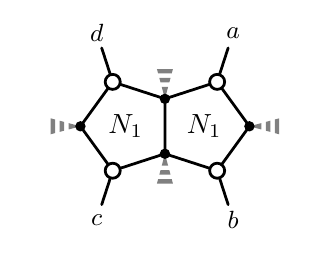
\begin{tikzpicture}[scale=\figScale,baseline=-2.45]\useasboundingbox ($(-7.5/3*\figScale,-1.5)$) rectangle ($(7.5/3*\figScale,1.5)$);\draw[int,line width=0.1,red,draw=none] ($(-7.5/3*\figScale,-1.5)$) rectangle ($(7.5/3*\figScale,1.5)$);\coordinate(v1) at ($(0,0)+(90:\edgeLen/2)$);\coordinate(v2)at($(v1)+(18:\edgeLen)$);\coordinate(v3)at($(v2)+(18-72:\edgeLen)$);\coordinate(v4)at($(v3)+(18-2*72:\edgeLen)$);\coordinate(v5)at($(v4)+(18-3*72:\edgeLen)$);\coordinate(v6)at($(v5)+(198-0*72:\edgeLen)$);\coordinate(v7)at($(v6)+(198-1*72:\edgeLen)$);\coordinate(v8)at($(v7)+(198-2*72:\edgeLen)$);
\draw[int](v1)--(v2)--(v3)--(v4)--(v5)--(v6)--(v7)--(v8)--(v1);\draw[int](v1)--(v5);\optLeg{(v1)}{90};\leg{(v2)}{72}{$a$};\optLeg{(v3)}{72-1*72};\leg{(v4)}{72-2*72}{$b$};\optLeg{(v5)}{-90};\leg{(v6)}{252-0*72}{$c$};\optLeg{(v7)}{252-1*72};\leg{(v8)}{252-2*72}{$d$};\foreach\a in {1,3,5,7}{\node at (v\a) [bdot]{};};\foreach\a in {2,4,6,8}{\node at (v\a) [wdot]{};};
\node at ($(\edgeLen/1.4,0)$) []{$N_1$};\node at ($(-\edgeLen/1.4,0)$) []{$N_1$};
\end{tikzpicture}}


\title{Algebraic letters and NMHV last entry conditions from $\bar{Q}$-equation}
\subtitle{\scriptsize Based on works with Song He and Zhenjie Li}
% \date{\today}
\date{}
\author{Chi Zhang}
\institute{Institute of Theoretical Physics, CAS}
 %\titlegraphic{\includegraphics[height=1.0cm]{logo.png}\hfill}

\begin{document}

\maketitle

\begin{frame}{Table of contents}
  \setbeamertemplate{section in toc}[sections numbered]
  \tableofcontents[hideallsubsections]
\end{frame}


\section{Review of $\mathcal{N}=4$ sYM and its amplitudes}
  


%\section{Symmetries of planar $\mathcal{N}=4$ sYM and $\bar{Q}$ equations}

  
  \begin{frame}{planar $\mathcal{N}=4$ sYM: Harmonic oscillator of QFT}
  \begin{enumerate}
    \item Solvable 4-dimensional QFT
    \item New mathematical structures 
    \item Fruitful playground for Feynman loop integrals
    \item SUSY cousin of QCD
  \end{enumerate}

\end{frame}


\begin{frame}{Field Content and Superamplitude}
    Simplicity of field content:  
\begin{itemize}
    \item 2 gauge bosons with $h=\pm 1$: \quad   $\lvert a\rangle ^{+1}, \lvert a\rangle^{-1}_{ABCD} $,
    \item 8 fermions with $h=\pm 1/2$:  \qquad \!\!\, $\lvert a\rangle_{A} ^{+1/2}, \lvert a\rangle^{-1/2}_{BCD} $,
    \item 6 scalars: \qquad \qquad \qquad \qquad  \quad\:  $\lvert a\rangle_{AB} ^{0}$.
\end{itemize}
Related by SUSY generators $Q_{A}^{\alpha}$ and $\tilde{Q}_{A}^{\dot{\alpha}}$,

grouped into a \alert{single} supermultiplet:
\begin{align*}
\lvert a\rangle &:= \exp (\tilde{Q}_{A}\cdot\tilde{\lambda}\cdot \tilde{\eta}^{A}) \lvert a\rangle ^{+} \\
&= \lvert a \rangle ^{+}+ \tilde{\eta}^{A}\lvert a\rangle_{A}^{1/2}+\cdots +\frac{1}{4!}\tilde{\eta}^{A}\tilde{\eta}^{B}\tilde{\eta}^{C}\tilde{\eta}^{D}\lvert a\rangle^{-}_{ABCD}
\end{align*}
We are considering the scattering of $n$ supermultiplets:
\[
A_{n}(\{p_{i},\tilde{\eta}_{i}\}) = \delta^{4}(P)\delta^{8}(Q)\bigl(\mathcal{A}_{n,0}(\{p_{i}\})+\mathcal{A}_{n,1}(\{p_{i},\tilde{\eta_{i}}\})+\cdots\bigr)
\]
\end{frame}



\begin{frame}[fragile]{Scattering Amplitude/Wilson loop duality} %Dual super conformal symmetries and notations

Amplitudes in planar $\mathcal{N}=4$ sYM enjoy not only superconformal symmetries, but also \alert{dual} superconformal symmetries, {\footnotesize[\textcolor{darkred}{Drummond,Henn,Smirnov,Sokatchev}]} which 
is manifest in a chiral superspace cooidnates $(x,\theta)$
\begin{align*}
   & \textcolor{limegreen}{x_{i}^{\alpha\dot{\alpha}}-x_{i+1}^{\alpha\dot{\alpha}}} = \lambda_{i}^{\alpha}\tilde{\lambda}_{i}^{\dot{\alpha}}
    = \textcolor{oceanboatblue}{p_{i}^{\mu}}\sigma_{\mu}^{\alpha\dot{\alpha}}, \qquad 
    \theta_{i}^{\alpha A}-\theta_{i+1}^{\alpha A} =\lambda_{i}^{\alpha}\tilde{\eta}_{i}^{A} \\
    & \text{planar poles:} \quad (p_{i}+p_{i+1}+\cdots+p_{j-1})^{2}=x_{ij}^{2}
\end{align*}

\begin{columns}
  \column{0.4\textwidth}
\scalebox{0.5}{
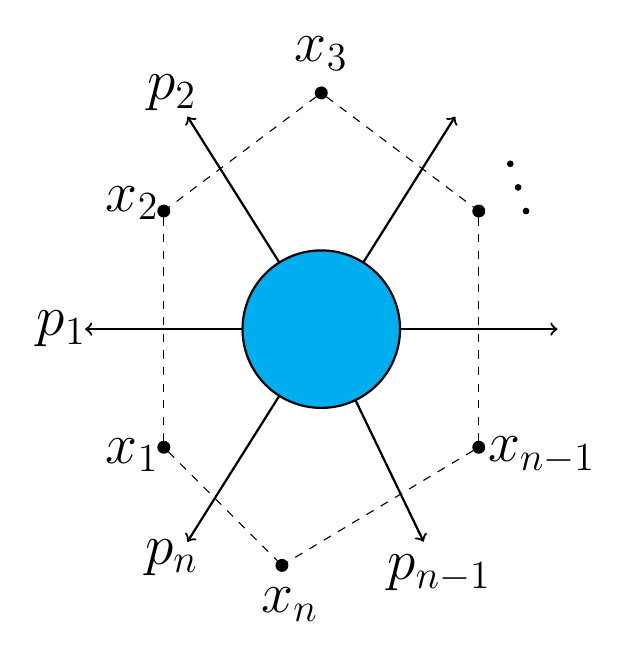
\begin{tikzpicture}
  \node (v2) at (-3,2.5) [circle,draw=black,fill=black,inner sep=0pt,minimum size=1.5mm]  {};
  \node (v1) at (-1,4) [circle,draw=black,fill=black,inner sep=0pt,minimum size=1.5mm] {};
  \node (v6) at (1,2.5) [circle,draw=black,fill=black,inner sep=0pt,minimum size=1.5mm] {};
  \node (v3) at (-3,-0.5) [circle,draw=black,fill=black,inner sep=0pt,minimum size=1.5mm] {};
  \node (v4) at (-1.5,-2) [circle,draw=black,fill=black,inner sep=0pt,minimum size=1.5mm] {};
  \node (v5) at (1,-0.5) [circle,draw=black,fill=black,inner sep=0pt,minimum size=1.5mm]  {};
  \draw[dashed]   (v1) -- (v2);
  \draw[dashed]  (v2)-- (v3);
  \draw[dashed]  (v3) -- (v4);
  \draw[dashed]  (v5) -- (v4);
  \draw[dashed]  (v6) -- (v5);
  \draw[dashed]  (v1) -- (v6);
  \node at (-3.4,2.6) {\huge $x_{2}$};
  \node at (-1,4.5) {\huge $x_{3}$};
  \node at (1.8,-0.6) {\huge $x_{n-1}$};
  \node at (-1.4,-2.5) {\huge $x_{n}$};
  \node at (-3.4,-0.6) {\huge $x_{1}$};
  \draw[->,thick] (-2,1)--(-4,1);
  \draw[->,thick] (-1,1)--(-2.7,3.7);
  \draw[->,thick] (-1,1)--(0.7,3.7);
  \draw[->,thick] (-1,1)--(2,1);
  \draw[->,thick] (-1,1)--(0.3,-1.7);
  \draw[->,thick] (-1,1)--(-2.7,-1.7);
  \filldraw[draw=black,fill=cyan,thick] (-1,1) ellipse (1 and 1);
  \node at (-4.3,1) {\huge $p_{1}$};
  \node at (-2.9,4.0) {\huge $p_{2}$};
  \node at (-2.9,-1.9) {\huge $p_{n}$};
  \node at (0.5,-2.1) {\huge $p_{n-1}$};
  \node at (1.4,3.1) [circle,draw=black,fill=black,inner sep=0pt,minimum size=0.7mm] {};
  \node at (1.5,2.8) [circle,draw=black,fill=black,inner sep=0pt,minimum size=0.7mm] {};
  \node at (1.6,2.5) [circle,draw=black,fill=black,inner sep=0pt,minimum size=0.7mm] {};
  \end{tikzpicture}
}

\column{0.6\textwidth}
In dual space, an amplitude become a light-like polygonal Wilson loop. 

\begin{equation*}
  \mathcal{A}_{n}(p_{1},p_{2},\cdots,p_{n}) \Leftrightarrow W_{n}(x_{1},\cdots,x_{n})
\end{equation*}



\end{columns}


% \begin{columns}
%  \column{0.7\textwidth}
% In dual space, an amplitude become a light-like polygonal Wilson loop which is invariant under conformal transformation:
% \begin{align*}
% I(x_{i}^{\alpha\dot{\alpha}}) &= \frac{x_{i}^{\alpha\dot{\alpha}}}{x_{i}^{2}} \\
% D(x_{i}^{\alpha\dot{\alpha}}) &= tx_{i}^{\alpha\dot{\alpha}} 
% \end{align*}
% \column{0.3\textwidth}

% \begin{tikzpicture}[thick,decoration={
%     markings,
%     mark=at position 0.5 with {\arrow{>}}}
%     ] 
%     \draw[postaction={decorate}] (0,0) node[below] {$ \textcolor{limegreen}{x_{1}}$} --(0,2) node[left=5pt,above] { $\textcolor{limegreen}{x_{2}}$} ;
%     \draw[postaction={decorate}] (0,2)--(1,3) node[above] {$ \textcolor{limegreen}{x_{3}}$} ;
%     \draw[postaction={decorate}] (1,3)--(2,2) node[right] {$ \textcolor{limegreen}{x_{4}}$};
%     \draw[postaction={decorate}] (2,2)--(2,1)node[right] {$ \textcolor{limegreen}{x_{5}}$};
%     \draw[postaction={decorate}] (2,1)--(0,0);
    
%     \node[fill, circle, inner sep=0pt,minimum size=3pt] at (0,0) {};
%     \node[fill, circle, inner sep=0pt,minimum size=3pt] at (0,2) {};
%     \node[fill, circle, inner sep=0pt,minimum size=3pt] at (1,3) {};
%     \node[fill, circle, inner sep=0pt,minimum size=3pt] at (2,2) {};
%     \node[fill, circle, inner sep=0pt,minimum size=3pt] at (2,1) {};
    
%     \draw (0,0.9) node[right]  {$ \textcolor{oceanboatblue}{p_{1}}$};
%     \draw (0.6,2.5) node[below]  {$ \textcolor{oceanboatblue}{p_{2}}$};
%     \draw (1.4,2.6) node[below]  {$ \textcolor{oceanboatblue}{p_{3}}$};
%     \draw (2,1.5) node[left]  {$ \textcolor{oceanboatblue}{p_{4}}$};
%      \draw (1,0.5) node[above]  {$ \textcolor{oceanboatblue}{p_{5}}$};
% \end{tikzpicture}


% \end{columns}

\end{frame}

\begin{frame}[fragile]{Superconformal and dual superconformal symmetries}

\begin{center}
  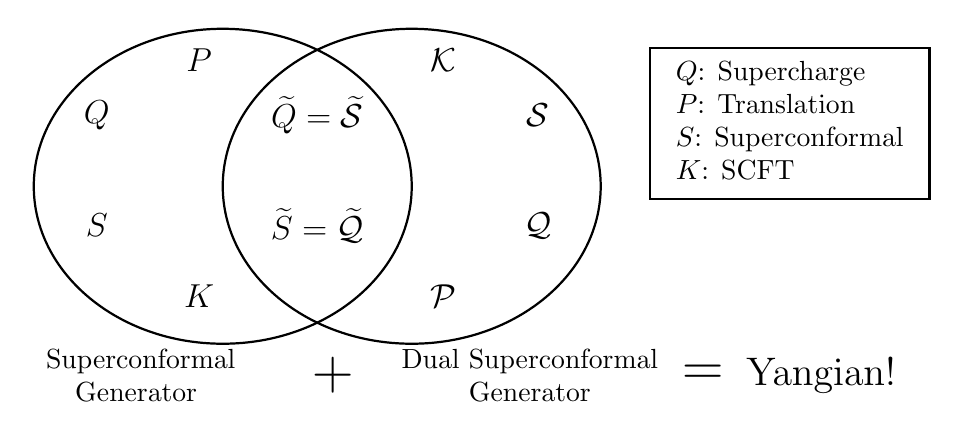
\begin{tikzpicture}[thick]
    \draw  (-2.4,0.4) node (v1) {};
    \draw  (v1) ellipse (2.4 and 2);
    \draw  (0,0.4) node (v2) {};
    \draw  (v2) ellipse (2.4 and 2);
    \node at (-1.2,1.3) {\large $\tilde{Q}=\tilde{\mathcal{S}}$};
    \node at (-1.2,-0.1) {\large $\tilde{S}=\tilde{\mathcal{Q}}$};
    \node at (-2.7,-1.0) {\large $K$};
    \node at (-2.7,2.0) {\large $P$};
    \node at (-4.0,1.3) {\large $Q$};
    \node at (-4.0,-0.1) {\large $S$};
    \node at (0.4,-1.0) {\large $\mathcal{P}$};
    \node at (0.4,2.0) {\large $\mathcal{K}$};
    \node at (1.6,1.3) {\large $\mathcal{S}$};
    \node at (1.6,-0.1) {\large $\mathcal{Q}$};
    \node at (-3.5,-2.0) [align=center] {\alert{ Superconformal} \\ \alert{Generator}};
    \node at (1.5,-2.0) [align=center] {\alert{Dual Superconformal} \\ \alert{Generator}};
    \node at (-1.0,-2.0) {\huge $+$};
    \node at (3.7,-2.0) {\huge $=$};
    \node at (5.2,-2.0) {\alert {\Large Yangian!}};
    \node at (4.8,1.2) [draw] {
    \begin{tabular}{l}
$Q$: Supercharge\\
$P$: Translation \\
$S$: Superconformal \\
$K$: SCFT \\
    \end{tabular}}; 
    \end{tikzpicture}
\end{center}
In terms of $\lambda$, $\tilde{\lambda}$, $x$, the generators are not linear realized:  
\begin{align*}
K_{\alpha\dot{\alpha}}=\sum_{i=1}^{n}\frac{\partial^{2}}{\partial\lambda_{i}^{\alpha}\partial\tilde{\lambda}_{i}^{\dot{\alpha}}}\:, \qquad 
\mathcal{K}^{\alpha\dot{\alpha}} =\sum_{i=1}^{n}\biggl[x_{i}^{\alpha\dot{\beta}}
x_{i}^{\beta\dot{\alpha}}\frac{\partial}{\partial x_{i}^{\beta\dot{\beta}}}+\cdots \biggr]
\end{align*}

\end{frame}


\begin{frame}[fragile]{Yangian and Grassmannian}
 (Dual) superconformal symmetry $\mathrm{SL}(4\vert 4)$ is linearly realized in terms of super (momentum) twistor
 \begin{align*}
 \mathcal{W}_{i}^{I}&=(W_{i}^{a}\vert \tilde{\eta}_{i}^{A}) := (\tilde{\mu}_{i}^{\alpha},\tilde{\lambda}_{i}\vert  \tilde{\eta}_{i}^{A}) \quad \text{by Fourier trans. } \smallint \exp(\mi\lambda_{i}\tilde{\mu}_{i}) \\
 \mathcal{Z}_{i}^{I}&=(Z_{i}^{a}\vert \chi_{i}^{A}):=(\lambda_{i}^{\alpha},x_{i}^{\alpha\dot{\alpha}}\lambda_{i\alpha}\vert\theta_{i}^{\alpha A}\lambda_{i\alpha}). \qquad {\footnotesize\text{[\textcolor{darkred}{Hodges}] }}
 \end{align*}
 For funture convenience, we introduce two basic invariants:
 \begin{align*}
     &\text{Pl\"{u}cker coordinate}:\quad \langle ijkl\rangle :=\varepsilon_{abcd}Z_{i}^{a}Z_{j}^{b}Z_{k}^{c}Z_{l}^{d}, \: 
    \biggl( x_{ij}^{2}=\frac{\langle i{-}1\,i\,j{-}1\,j\rangle}{\langle i{-}1\,i\rangle\langle j{-}1\,j\rangle}\biggr) \\ 
     &\text{R invariant}:\quad [i\,j\,k\,l\,m]:=\frac{\delta^{0\vert 4}(\chi_{i}^{A}\langle jklm\rangle+\text{cyclic})}{\langle ijkl\rangle\langle jklm\rangle\langle klmi\rangle\langle lmij\rangle\langle mijk\rangle} \:,
 \end{align*}
where R invariants are the first kind of non-trivial Yangian invariant!
%  \footnotesize Tree amplitudes satisfy 
%  \[
%   G R_{n}^{\text{tree}} =0 \,\qquad A_{n}^{\text{tree}}= \frac{\delta^{4}(P)\delta^{8}(Q)}{\langle 12\rangle\cdots \langle n1\rangle }
%   R_{n}^{\text{tree}}
%  \]
%  where the chiral half of these generators 
%  \begin{equation*}
%      \bar{Q}_{a}^{A}= \sum_{i}\chi_{i}^{A}\frac{\partial}{\partial Z_{i}^{a}}
%  \end{equation*}
% play an important role in the calculation of amplitudes.
\end{frame}

\begin{frame}
\footnotesize
In terms of (momentum) twistor, Yangian symmetries are generated by
\begin{align*}
  \text{level 0:   }& \sum_{i=1}^{n}G_{i}^{I}{}_{J}\:, \\
  \text{level 1:   }& \sum_{i<j}^{n}(-1)^{\lvert K\rvert} [G_{i}^{I}{}_{K}G_{j}^{K}{}_{J}-(i\leftrightarrow j)]  \:, \cdots
\end{align*}
where 
\begin{equation*}
  G_{i}^{I}{}_{J}= \mathcal{Z}_{i}^{I}\frac{\partial}{\partial \mathcal{Z}_{i}^{J}}\quad \text{or}\quad   \mathcal{W}_{i}^{I}\frac{\partial}{\partial \mathcal{W}_{i}^{J}}
\end{equation*}
Then the Yangian invariants can be proven to be Grassmannian integrals [{\textcolor{darkred}{Arkani-Hamed, Drummond,$\cdots$}}]
\begin{equation*}
  Y_{n,k}^{(\gamma)}(\mathcal{Z})=\int_{\gamma} \frac{\dif^{k\times n} C}{\operatorname{vol}\mathrm{GL}(k)} \frac{\delta^{4k\vert 4k}(C \cdot \mathcal{Z})}{(1\cdots k)\cdots (n\cdots k-1)} \label{grassforYangian}
\end{equation*}
or
\begin{equation*}
  \mathcal{L}_{n,k}^{(\gamma)}(\lambda,\tilde{\lambda},\tilde{\eta}) = \int_{\gamma} \frac{\dif^{K\times n}C}{\operatorname{vol}\mathrm{GL}(K)}
  \frac{\delta^{2K}(C\cdot \tilde{\lambda})\delta^{2(n-K)}(C^{\perp}\cdot \lambda)\delta^{4K}(C\cdot \tilde{\eta})}{(1\cdots K)\cdots (n\cdots K{-}1)}  \quad (K:=k+2)\:.\label{grassforLS}
\end{equation*}
\end{frame}

\begin{frame}{Yangian invariant as leading singularities}
When Yangian invariants are expressed as Grassmannian integrals, they are associated with a diagrammatic representation {\footnotesize[\textcolor{darkred}{Arkani-Hamed, Bourjaily, Cachazo, Goncharov, Postnikov, Trnka}]}:
\begin{columns}
  \column{0.3\textwidth}
  \hfill \begin{center}
    \raisebox{-51pt}{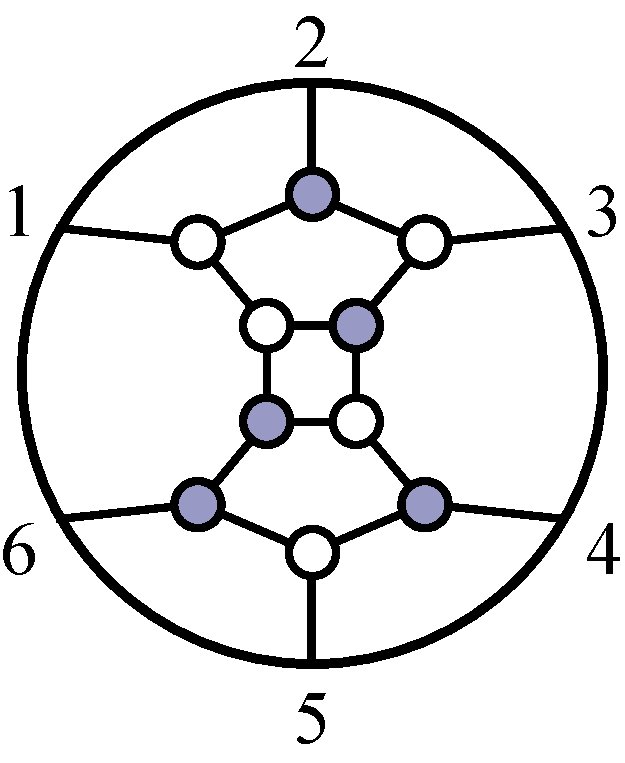
\includegraphics[scale=0.25]{plabic}} 
  \end{center}
  \column{0.6\textwidth}
  \begin{align*}
   \text{ black/white vertex} &\to \text{ 3-pt MHV/$\overline{\text{MHV}}$} \\
    \text{propagator } &\to   \int \frac{\dif^{2}\lambda_{I}\dif^{2}\tilde{\lambda}_{I} \dif^{4}\tilde{\eta}_{I}}{\mathrm{GL}(1)} 
  \end{align*}
\end{columns}
Yangian invariants are leading singularities of loop integrand! By generalized unitarity method,
\begin{equation*}
  \mathcal{A}_{n,k,L}= \sum Y_{n,k} \times \text{scalar integrals} \:.
\end{equation*}
  
\end{frame}

\begin{frame}{General structure of loop amplitudes in planar $\mathcal{N}=4$ sYM}

Recall that $A_{n,k}=\sum Y_{n,k}\times \alert{\text{scalar integral}  }.$
   \begin{itemize}
       \item The dual conformal invariance of amplitudes is broken at the loop-level due to the infrared divergence.
       \item This symmtery can be restored by subtracting the infrared part $A_{n}^{\text{BDS}}$ {\footnotesize[\textcolor{darkred}{Bern, Dixon, Smirnov}]}.
   \end{itemize}
\begin{equation*}
    A_{n}= \underbrace{A_{n}^{\text{BDS}}}_{IR}\times \overbrace{\underbrace{\exp (R_{n})}_{\substack{\text{Remainder}\\ \text{function}}}
    \times \underbrace{\Bigl(1+ \mathcal{P}_{n}^{\text{NMHV}}+\cdots+\mathcal{P}_{n}^{\overline{\text{MHV}}} \Bigr)}_{\text{Ratio functions}}}^{\text{finite functions of dual conformal invariants}}
\end{equation*}
For example, $R_{6}$ will be a function of $u=\frac{\langle 1234\rangle\langle 4561\rangle}{\langle 1245\rangle\langle 3461\rangle}$, $v=\frac{\langle 3456\rangle\langle 6123\rangle}{\langle 3461\rangle\langle 5623\rangle}$, $w=\frac{\langle 5612 \rangle\langle 2345\rangle}{\langle 5623\rangle\langle 1245\rangle}.$
\\
We are interested in the function $R_{n,1}^{(2)}=\bigl(\exp(R_{n})\mathcal{P}_{n}^{\text{NMHV}}\bigr)^{(2)}$ 

\textcolor{hblue}{\footnotesize{In the following, we will denote $\exp(R_{n})\mathcal{P}_{n}^{\text{N}^{k}\text{MHV}}$ by $R_{n,k}$}}
\end{frame}



\begin{frame}{Poles and Cuts}
  In general, the BDS-normalized amplitudes $R_{n,k}$ can be written as 
 \begin{equation*}
   R_{n,k}^{(L)} =\sum_{\alpha} Y_{n,k}^{\alpha}F_{\alpha}^{(2L)} 
 \end{equation*}
 where $Y_{n,k}$ are Yangian invariants %(which means $\bar{Q}Y_{n,k}=0$)
 \begin{itemize}
   \item $Y_{n,k}$ bear the pole structure of amplitudes,
   \item $Y_{n,k}$ are \alert{independent of loop-integral},
   \item $F$ are transcendental functions of cross-ratios bearing the cut structure of amplitudes.
 \end{itemize} 
 %which bear the \alert{cut} structure of amplitudes and are expected to be generalized polylogarithms of weight $2L$ at $L$-loop level for MHV and NMHV cases.
%For MHV and NMHV, $F^{(2L)}$ are believe to be just Polylogarithms of weight $\alert{2L}$
For MHV and NMHV amplitudes, $F$ are believe to be just polylogarithms of weight $2L$  {\footnotesize[\textcolor{darkred}{Arkani-Hamed, Bourjaily, Cachazo, Goncharov, Postnikov, Trnka}]}.
 \end{frame}

\begin{frame}{Polylogarithms and Symbol}
Polylogarithms [\textcolor{darkred}{Goncharov}] of weight $2L$ are $2L$-fold iterated integrals.
\begin{equation*}
   F^{(2L)} = \int_{\gamma} \mathrm{d}\log s_{1} \circ\cdots\circ \mathrm{d}\log s_{2L} 
\end{equation*}
This define the \alert{symbol} of $F$:
\begin{equation*}
  \mathcal{S}(F^{(2L)}):= s_{1}\otimes \cdots \otimes s_{2L}
\end{equation*}
where $s_{i}$ are called \alert{symbol letters}.

\only<1>{Some example:
\begin{align*}
  \mathcal{S}(\log x\log y)= x\otimes y+ y\otimes x, \quad
  \mathcal{S}(\operatorname{Li}_{2}(z))=-\bigl((1-z)\otimes z\bigr)
\end{align*} The \alert{first entries} of symbol indicate the locus of cuts of $F$}

\only<2>{\alert{Last entries} of Symbol:
\begin{gather*}
\mathcal{S}(\mathrm{d} F^{(2L)}) =  s_{1}\otimes \cdots \otimes s_{2L-1} \mathrm{d}\log s_{2L}
\end{gather*}
}
\end{frame}


\begin{frame}[t]{Boostrap}


 \tikzstyle{scorestars}=[star, star points=5, star point ratio=2.25, draw, inner sep=1.3pt, anchor=outer point 3]%

\begin{columns}
  \column{0.5\textwidth}
 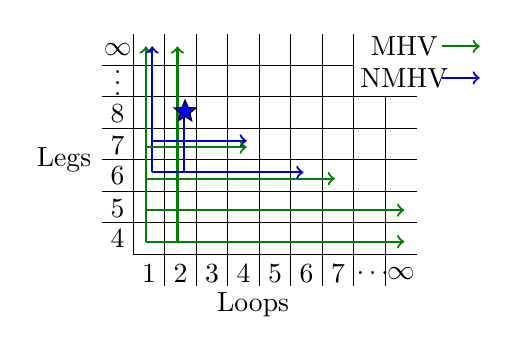
\begin{tikzpicture}[scale=0.8]
\node at (-3.6,0) {\text{Legs}};
\node at (-0.6,-2.3) {\text{Loops}};
\node at (1.8,1.3) {\text{NMHV}};
\node at (1.8,1.8) {\text{MHV}};
\draw[thick,blue!80!black,->] (2.4,1.3) -- (3.0,1.3);
\draw[thick,green!50!black,->] (2.4,1.8) -- (3.0,1.8);
\draw (-2.5,2) -- (-2.5,-1.5) -- (2,-1.5);
\draw (-3,-1) -- (2,-1);
\draw (-3,-0.5) -- (2,-0.5);
\draw (-3,0) -- (2,0);
\draw (-3,0.5) -- (2,0.5);
\draw (-3,1) -- (2,1);
\draw (-3,1.5) -- (1,1.5);
\draw (-2,2) -- (-2,-2);
\draw (-1.5,2) -- (-1.5,-2);
\draw (-1,2) -- (-1,-2);
\draw (-0.5,2) -- (-0.5,-2);
\draw (0,2) -- (0,-2);
\draw (0.5,2) -- (0.5,-2);
\draw (1,2) -- (1,-2);
\node at (-2.75,1.75) {$\infty$};
\node at (-2.75,1.35) {$\vdots$};
\node at (-2.75,0.73) {$8$};
\node at (-2.75,0.23) {$7$};
\node at (-2.75,-0.25) {$6$};
\node at (-2.75,-0.77) {$5$};
\node at (-2.75,-1.25) {$4$};
\node at (1.75,-1.8) {$\infty$};
\node at (01.3,-1.8) {$\dots$};
\node at (0.75,-1.8) {$7$};
\node at (0.25,-1.8) {$6$};
\node at (-0.25,-1.8) {$5$};
\node at (-0.75,-1.8) {$4$};
\node at (-1.25,-1.8) {$3$};
\node at (-1.75,-1.8) {$2$};
\node at (-2.25,-1.8) {$1$};
\draw (1.5,-2) -- (1.5,1.0);
\draw[thick,green!50!black,->] (-2.3,-1.3) -- (-2.3,1.8);
\draw[thick,green!50!black,->] (-2.3,-1.3) -- (1.8,-1.3);
\draw[thick,green!50!black,->] (-2.3,-0.8) -- (1.8,-0.8);
\draw[thick,green!50!black,->] (-2.3,-0.3) -- (0.7,-0.3);
\draw[thick,green!50!black,->] (-1.8,-1.3) -- (-1.8,1.8);
\draw[thick,blue!80!black,->] (-2.2,-0.2) -- (0.2,-0.2);
\draw[thick,blue!80!black,->] (-2.2,-0.2) -- (-2.2,1.8);
\draw[thick,blue!80!black,->] (-2.2,0.3) -- (-0.7,0.3);
\draw[thick,green!50!black,->] (-2.3,0.2) -- (-0.7,0.2);
\draw[thick,blue!80!black] (-1.7,-0.2) -- (-1.7,0.7);
%\draw[thick,blue!80!black,densely dashed,->] (-1.7,0.7) -- (-1.7,1.8);
%\draw[thick,green!50!black] (-1.3,-0.2) -- (-1.3,0.7);
%\draw[thick,green!50!black,densely dashed,->] (-1.3,0.7) -- (-1.3,1.8);
\node[fill=blue,star, star points=5, star point ratio=2.25, draw, inner sep=1.3pt, anchor=outer point 3] at (-1.8,0.6) {};

\end{tikzpicture}

\column{0.5\textwidth}
The alphabets (collection of all possible letters) for hexagon and heptagon are  constrained by \alert{finite-type} cluster algebras $G(4,6)$ and $G(4,7)$

\end{columns} 
 
{\footnotesize  [\textcolor{darkred}{Bern, Caron-Huot, Dixon, Drummond,\ldots}]}

For more than seven particles, symbol alphabets are not well understood
\begin{itemize}
  \item  $G(4,n\geq 8)$ are \alert{infinite-type} cluster algebras.
  \item \alert{Square roots} appear in symbol letters even at one-loop in N$^{2}$MHV amplitudes
\end{itemize}
We will call the letters involving square roots as \alert{algebraic letters}.
\end{frame}


\section{$\bar{Q}$-equation and last entry conditions}

\begin{frame}{Dual superconformal anomaly and $\bar{Q}$ equations}
% Since we are considering the scattering of massless particles. The dual conformal invariance of amplitudes is broken at the loop-level due to the infrared divergence.

%This symmtery can be restored by subtracting the infrared part $A_{n}^{\text{BDS}}$.
BDS-normalized amplitudes $R_{n,k}$ are dual conformal invariants, but $R_{n,k}$ are \alert{not} dual superconformal invariants, they have anomalies under the symmetries generated by
\begin{equation*}
  \bar{Q}_{a}^{A}=\sum_{i}\chi_{i}^{A}\frac{\partial}{\partial Z_{i}^{a}}
\end{equation*}

\only<1>{An OPE analysis tell us the action of $\bar{Q}$ on $R_{n,k}$ can be given by an integral over higher-point amplitudes {\footnotesize[\textcolor{darkred}{Caron-Huot, He}]}
\begin{align*}
    \bar{Q}_{a}^{A}R_{n,k}=\frac{\Gamma_{\text{cusp}}}{4}\int_{\tau=0}^{\tau=\infty} \oint_{\epsilon=0}\Bigl(\mathrm{d}^{2\vert3}\mathcal{Z}_{n+1}\Bigr)_{a}^{A}\,[R_{n+1,k+1}-R_{n,k}R_{n+1,1}^{\text{tree}}] +\text{cyclic}
\end{align*}
where the particle $n{+}1$ is added in a collinear limit
\begin{equation*}
    \mathcal{Z}_{n+1}=\mathcal{Z}_{n}-\epsilon \mathcal{Z}_{n-1}+\frac{\langle n{-}1\,n\,2\,3\rangle}{\langle n \,1\,2\,3\rangle} \epsilon\tau \mathcal{Z}_{1}+\frac{\langle n{-}2\,n{-}1\,n\,1\rangle}{\langle n{-}2 \,n{-}1\,2\,1\rangle}\epsilon^{2}\mathcal{Z}_{2}
\end{equation*}
}
\only<2>{Perturbatively, this equation becomes
\begin{align*}
    \bar{Q}_{a}^{A}R^{(L)}_{n,k}=\int_{\tau=0}^{\tau=\infty} \oint_{\epsilon=0}\Bigl(\mathrm{d}^{2\vert3}\mathcal{Z}_{n+1}\Bigr)_{a}^{A}\,[R^{(L-1)}_{n+1,k+1}-R_{n,k}^{(L-1)}R_{n+1,1}^{\text{tree}}] +\text{cyclic}
\end{align*}
where the particle $n{+}1$ is added in a collinear limit
\begin{equation*}
    \mathcal{Z}_{n+1}=\mathcal{Z}_{n}-\epsilon \mathcal{Z}_{n-1}+ \underbrace{\frac{\langle n{-}1\,n\,2\,3\rangle}{\langle n \,1\,2\,3\rangle}}_{C}\epsilon\tau \mathcal{Z}_{1}+\underbrace{\frac{\langle n{-}2\,n{-}1\,n\,1\rangle}{\langle n{-}2 \,n{-}1\,2\,1\rangle}}_{C'}\epsilon^{2}\mathcal{Z}_{2}
\end{equation*}
}
    
\end{frame}


\begin{frame}{The integral measure}
    The basic operation $\int (\dif^{2\vert 3} \mathcal{Z}_{n+1})_{a}^{A}$ consist of bosonic part and fermionic part:
  \begin{align*}
    \bigl(\mathrm{d}^{2\vert 3}\mathcal{Z}_{n+1}\bigr)_{a}^{A}
    \begin{cases}
      \varepsilon_{abcd}Z_{n+1}^{b}\mathrm{d}Z_{n+1}^{c}\mathrm{d}Z_{n+1}^{d} = C(\bar{n})_{a}\epsilon\dif\epsilon \dif\tau &  (\text{Bosonic Part})  \\
      \\
      (\dif^{3} \chi_{n+1})^{A}  &(\text{Fermionic Part})
    \end{cases}
  \end{align*}
where $(\bar{n})_{a}:=\varepsilon_{abcd}Z_{n-1}^{b}Z_{n}^{c}Z_{1}^{d} $

The order of performing integral:
\begin{itemize}
  \item Fermionic integral $(\dif^{3} \chi_{n+1})^{A}$ 
  \item The substitution $ \mathcal{Z}_{n+1}\to \mathcal{Z}_{n}-\epsilon \mathcal{Z}_{n-1}+C\epsilon\tau \mathcal{Z}_{1}+C^{\prime}\epsilon^{2}\mathcal{Z}_{2} $
  \item Take the residue $\oint_{\epsilon=0}\dif\epsilon$ (\alert{Collinear limit})
  \item  1-D integral $\int_{0}^{\infty}\dif\tau$ (\alert{Real integral})
\end{itemize}
\end{frame}

%\section{Structures of Loop amplitudes and action of $\bar{Q}$ }


\begin{frame}[t]{$\bar{Q}$ as Differenial}
\only<1-2>{
Due to dual conformal invariance(DCI), $F$ are functions of cross ratios of Pl\"{u}cker coordinates. Since $F$ are expected to be polylogarithms, they satisfy
\begin{equation*}
  \dif F^{(2L)} = \sum_{\beta} F^{(2L-1)}_{\beta}\dif \log s_{\beta} \qquad  \biggl( \dif:=\sum_{i}\dif Z_{i}\frac{\partial}{\partial Z_{i}}\biggr)
\end{equation*}}
\only<2>{
Thus, the action of $\bar{Q}$ on $R_{n,k}^{(L)}$ gives
\begin{equation*}
 \bar{Q}R_{n,k}^{(L)} = \sum_{\alpha,\beta} Y_{n,k}^{\alpha}
 F_{\alpha,\beta}^{(2L-1)}\bar{Q}\log s_{\alpha,\beta}   \qquad  \biggl( \bar{Q}:=\sum_{i} \chi_{i}\frac{\partial}{\partial Z_{i}}\biggr)
\end{equation*}
where $s_{\alpha,\beta}$ are some DCI of Pl\"{u}cker coordinates and referred to the \alert{last entries} of amplitudes}

\end{frame}

\begin{frame}{Kernel of $\bar{Q}$}
  
$\bar{Q}$-equation can not determine N$^{2}$MHV amplitudes on its own due to the non-trivial dependence of its kernel on $k$:

\begin{itemize}
  \setlength{\itemsep}{20pt}
  \item For $k=0$, the kernel of $\bar{Q}$ is trivial
  \item For $k=1$, it's non-trivial, but has no space of \alert{DCI} functions
  \item For $k\geq 2$, it's non-trivial, and it indeed contains \alert{DCI} functions.
\end{itemize}

By also considering \alert{$Q^{(1)}$ equations}, N$^{k\geq 2}$MHV amplitudes can be fixed uniquely up to some Yangian invariants.
\end{frame}




\begin{frame}[t]{RHS of $\bar{Q}$ equations}

Now let us consider the RHS of $\bar{Q}$ equation:\begin{align*}
  \int_{\tau=0}^{\tau=\infty} \oint_{\epsilon=0}\Bigl(\mathrm{d}^{2\vert3}\mathcal{Z}_{n+1}\Bigr)_{a}^{A}\,[R^{(L-1)}_{n+1,k+1}-\underbrace{R_{n,k}^{(L-1)}R_{n+1,1}^{\text{tree}}}_{\text{trivial}}] +\text{cyclic}
\end{align*}
\only<1-2>{The first step:
\begin{flalign*}
 R_{n+1,k+1}^{{(L-1)}}\begin{cases}
  Y_{n+1,k+1} &\xrightarrow[]{C(\bar{n})_{a}\oint_{\epsilon=0}\epsilon\dif\epsilon\dif^{3}\chi_{n+1}}\sum_{I,J}Y_{n,k}^{I,J}\bar{Q}\log\frac{\langle\bar{n}I\rangle}{\langle\bar{n}J\rangle}\dif \log f_{I,J}(\tau)\\
  F^{(2L-2)}&\xrightarrow[]{Z_{n+1}\to Z_{n}-\epsilon Z_{n-1}+\cdots} F^{(2L-2)}(\tau,\epsilon\to0)
  \end{cases}
\end{flalign*} }
\only<1>
{The second step:
\begin{equation*}
  \int_{0}^{\infty} \dif \log f_{I,J}(\tau)F^{(2L-2)}(\tau,\epsilon\to0) = F^{(2L-1)}
\end{equation*}
where $f_{I,J}(\tau)$ are rational functions of $\tau$ (\alert{with some exceptions discussed later})}
\only<2>{
The operation $C(\bar{n})_{a}\oint_{\epsilon=0}\epsilon\dif\epsilon\dif^{3}\chi_{n+1}$ is independent of loop order which gives last entry conditions on amplitudes.

For $R$ invariants, the operation gives the well known {\footnotesize{[\textcolor{darkred}{Caron-Huot}]}}
\begin{flalign*}
  {\text{\alert{MHV last entries}}}: \qquad  \bar{Q}\log \frac{\langle\bar{n}i\rangle}{\langle\bar{n}j\rangle} \qquad \qquad 
\end{flalign*}
}
\end{frame}


\begin{frame}[t]{N$^{2}$MHV Yangian invariants}


The N$^{2}$MHV Yangian invariants have already been classified. {\footnotesize[\textcolor{darkred}{Arkani-Hamed, Bourjaily, Cachazo, Goncharov, Postnikov, Trnka}]}

They are 
\begin{columns}
  \column{0.5\textwidth}
  \tiny
  \begin{align*}
    Y^{(2)}_1 &= [1,2,(23)\cap (456), (234) \cap (56) , 6] [2,3,4,5,6] \\
    \nonumber
    Y^{(2)}_2 &= [1,2,(34) \cap (567), (345) \cap (67), 7] [3,4,5,6,7] \\
    \nonumber
    Y^{(2)}_3 &= [1,2,3,(345) \cap (67), 7] [3,4,5,6,7] \\
    \nonumber
    Y^{(2)}_4 &= [1,2,3,(456) \cap (78), 8] [4,5,6,7,8] \\
    \nonumber
    Y^{(2)}_5 &= [1,2,3,4,8] [4,5,6,7,8] \\
    \nonumber
    Y^{(2)}_6 &= [1,2,3,(45) \cap (678), 8] [4,5,6,7,8] \\
    Y^{(2)}_7 &= [1,2,3,(45) \cap (678), (456) \cap (78)] [4,5,6,7,8]
  \end{align*}
  \column{0.5\textwidth}
  \tiny
  \begin{align*}
    Y^{(2)}_8 &= [1,2,3,4,(456) \cap (78)] [4,5,6,7,8] \\
    \nonumber
    Y^{(2)}_9 &= [1,2,3,4,9] [5,6,7,8,9] \\
    \nonumber
    Y^{(2)}_{10}&=[1,2,3,4,(567) \cap (89)] [5,6,7,8,9] \\
    \nonumber
    Y^{(2)}_{11}&=[1,2,3,4,(56) \cap (789)] [5,6,7,8,9] \\
    \nonumber
    Y^{(2)}_{12}&= \varphi 
    [1,2,3,(45) \cap (789) , (46) \cap (789)] [(45) \cap (123), (46) \cap (123), 7,8,9] \\
    Y^{(2)}_{13}&=[1,2,3,4,5][6,7,8,9,10] \\
    Y^{(2)}_{14}&=\psi [A,1,2,3,4][B,5,6,7,8]
    \nonumber
  \end{align*}
\end{columns}
  where
  \begin{align*}
  (i j) \cap (k l m ) = \mathcal{Z}_i \langle j\, k\, l\, m \rangle - \mathcal{Z}_j \langle i\, k \, l\, m \rangle
  \end{align*}

\end{frame}

\begin{frame}[t]{NMHV last entry conditions}
  For N$^{2}$MHV yangian invariants, this operation gives three kinds of last entries \\
\footnotesize{
1.
\begin{flalign*}
   [i\,j\,k\,l\,m] \bar{Q}\log\frac{\langle\bar{n}a\rangle}{\langle\bar{n}b\rangle}
\end{flalign*}
2.
\begin{align*}
  &[1\,i_{1}\,i_{2}\,i_{3}\,i_{4}]\,\bar{Q}\log\frac{\langle 1(n{-}1\,n)(i_{1}\,i_{2})(i_{3}\,i_{4})\rangle}{\langle\bar{n}i_{1}\rangle\langle1i_{2}i_{3}i_{4}\rangle} \:,  \quad 
  [i_{1}\,i_{2}\,i_{3}\,i_{4}\,n{-}1]\,\bar{Q}\log\frac{\langle n{-}1(n\,1)(i_{1}\,i_{2})(i_{3}\,i_{4})\rangle}{\langle\bar{n}i_{1}\rangle\langle n{-}1\,i_{2}i_{3}i_{4}\rangle} \\
  &[i_{1}\,i_{2}\,i_{3}\,i_{4}\,n]\,\bar{Q}\log\frac{\langle n(1\,n{-1})(i_{1}\,i_{2})(i_{3}\,i_{4})\rangle}{\langle\bar{n}i_{1}\rangle\langle n\,i_{2}i_{3}i_{4}\rangle} \quad\text{with} \,1<i_{1}<i_{2}<i_{3}<i_{4}<n{-}1 \nonumber
\end{align*}
where $\langle a(bc)(de)(fg)\rangle :=\langle abde\rangle\langle acfg\rangle -\langle acde\rangle\langle abfg\rangle$}

3. \begin{equation*}
  [i_{1}\,i_{2}\,i_{3}\,i_{4}\,i_{5}]\,\bar{Q}\log\frac{\langle \bar{n}(i_{1}i_{2})\cap(i_{3}i_{4}i_{5})\rangle }{\langle \bar{n}i_{1}\rangle \langle i_{2}i_{3}i_{4}i_{5}\rangle } \:, \:\: [i_{1}\,i_{2}\,i_{3}\,i_{4}\,i_{5}]\,\bar{Q}\log\frac{\langle \bar{n}(i_{1}i_{2}i_{3})\cap(i_{4}i_{5})\rangle }{\langle \bar{n}i_{1}\rangle \langle i_{2}i_{3}i_{4}i_{5}\rangle } \:,
\end{equation*}
with $1<i_{1}<i_{2}<i_{3}<i_{4}<i_{5}<n$
\end{frame}


% \begin{frame}[fragile,t]{Why octagon?}
  
% The surprise simplicity of $6$ and $7$-point amplitudes:
% \begin{itemize}
%   \item  The symbol alphabet for six-particle kinematics consists of 9 letters, which correspond to cluster algebra $G(4,6)$
%   \item  The symbol alphabet for seven-particle kinematics consists of 42 letters, which correspond to cluster algebra $G(4,7)$
% \end{itemize}
% With further physical constrains on the iterated structure of cuts, the 6-point amplitude has been determined through 7 loop for MHV and 6 loop for NMHV, the 7-point amplitude has been determined through 4 loop for both MHV and NMHV. [\textcolor{darkred}{Caron-Huot, Dixon, Drummond,\ldots}]

% For more than seven particles, symbol alphabets are not well understood
% \begin{itemize}
%   \item  $G(4,n\geq 8)$ are infinite-type cluster algebras.
%   \item algebraic roots appear in symbol letters even at one-loop in N$^{2}$MHV
%   amplitudes
% \end{itemize}

% \end{frame}

\section{Algebraic letters in two-loop NMHV amplitudes}

\begin{frame}[t]{Input}
To compute the 2-loop NMHV $n$ point BDS-normalized amplitude, we need the input of the one-loop N$^{2}$MHV BDS-normalized amplitude $R_{n+1,2}^{(1)}$, which can be obtained from the chiral/scalar box expansion {\footnotesize[\textcolor{darkred}{Bourjaily, Caron-Huot, Trnka}]}:
\begin{equation*}
  R_{n+1,2}^{(1)} =\sum_{a<b<c<d} (f_{a,b,c,d}-R_{n+1,2}^{\text{tree}} f_{a,b,c,d}^{\text{MHV}})\mathcal{I}_{a,b,c,d}^{\text{fin}}
\end{equation*}
where
\begin{itemize}
  \item $f_{a,b,c,d}$ are linear combinations of N$^{2}$MHV yangian invariants
  \item $f_{a,b,c,d}^{\text{MHV}}$ are either 1 or 0
  \item $\mathcal{I}_{a,b,c,d}^{fin}$ denote the finite part of DCI-regulated box integrals
\end{itemize}

\end{frame}

\begin{frame}[t]{Four-mass box}
The most generic term in box expansion:\\[5pt]
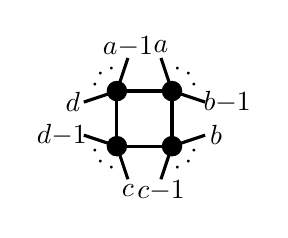
\begin{tikzpicture}[baseline={([yshift=-.5ex]current bounding box.center)},scale=0.7]
  \node[fill=black,circle,draw=black, inner sep=0pt,minimum size=7pt] at (-2,0) {};
  \node[fill=black,circle,draw=black, inner sep=0pt,minimum size=7pt] at (-2,-1) {};
  \node[fill=black,circle,draw=black, inner sep=0pt,minimum size=7pt] at (-1,-1) {};
  \node[fill=black,circle,draw=black, inner sep=0pt,minimum size=7pt] at (-1,0) {};
  \draw[line width=0.4mm] (-2,0) -- (-2,-1) -- (-1,-1) -- (-1,0) -- cycle;
  \draw[line width=0.4mm] (-2.6,-0.8) -- (-2,-1);
  \draw[line width=0.4mm] (-2,-1) -- (-1.8,-1.6);
  \draw[line width=0.4mm] (-1,-1) -- (-0.4,-0.8);
  \draw[line width=0.4mm] (-1,-1) -- (-1.2,-1.6);
  \draw[line width=0.4mm] (-2.6,-0.2) -- (-2,0);
  \draw[line width=0.4mm] (-1.8,0.6) -- (-2,0);
  \draw[line width=0.4mm] (-1.2,0.6) -- (-1,0);
  \draw[line width=0.4mm] (-1,0) -- (-0.4,-0.2);
  \node at (-1.2,0.8) {$a$};
  \node at (0,-0.2) {$b{-}1$};
  \node at (-0.2,-0.8) {$b$};
  \node at (-1.2,-1.8) {$c{-}1$};
  \node at (-1.8,-1.8) {$c$};
  \node at (-3,-0.8) {$d{-}1$};
  \node at (-2.8,-0.2) {$d$};
  \node at (-1.8,0.8) {$a{-}1$};
  \node at (-2.4,0.1) {$\cdot$};
  \node at (-2.3,0.3) {$\cdot$};
  \node at (-2.1,0.4) {$\cdot$};
  \node at (-0.9,-1.4) {$\cdot$};
  \node at (-0.7,-1.3) {$\cdot$};
  \node at (-0.6,-1.1) {$\cdot$};
  \node at (-0.6,0.1) {$\cdot$};
  \node at (-0.7,0.3) {$\cdot$};
  \node at (-0.9,0.4) {$\cdot$};
  \node at (-2.4,-1.1) {$\cdot$};
  \node at (-2.3,-1.3) {$\cdot$};
  \node at (-2.1,-1.4) {$\cdot$};
\end{tikzpicture}
$ \scriptsize \displaystyle
  \begin{cases}\displaystyle
      x_{ab}^2 := \frac{\langle a{-}1\,a\,b{-}1\,b\rangle}{\langle a{-}1\,a\rangle\langle b{-}1\,b\rangle}=(p_{a}+\cdots + p_{b-1})^{2},\\[12pt]
      u=\displaystyle\frac{x_{ad}^{2}x_{bc}^{2}}{x_{ac}^{2}x_{bd}^{2}}=z\bar{z},\quad v=\displaystyle\frac{x_{ab}^{2}x_{cd}^{2}}{x_{ac}^{2}x_{bd}^{2}}=(1-z)(1-\bar{z}),\\[12pt]
      \Delta_{abcd} =\sqrt{(1{-}u{-}v)^{2}-4uv}
  \end{cases}
$

For such a box, 
\begin{align*}
  f_{a,b,c,d} &= \frac{1-u-v\pm\Delta}{2\Delta}[\alpha_{\pm},b{-1},b,c-1,c][\delta_{\pm},d{-1},d,a{-}1,a] \\
  \mathcal{I}_{a,b,c,d}^{\text{fin}}&= \operatorname{Li}_{2}(z)-\operatorname{Li}_{2}(\bar{z})+\frac{1}{2}\log(z\bar{z})\log{\frac{1-z}{1-\bar{z}}}
\end{align*}
where $\alpha_{\pm}$ and $\delta_{\pm}$ are two solutions of Schubert problem $\alpha=(a{-}1 \,a)\cap (d\,d{-}1\,\gamma)$, $\gamma=(c{-}1 \,c)\cap (b\,b{-}1\,\alpha)$

\uncover<2>{The square root will disappear when one mass corner become massless, {\it e.g.} $b=a{+1}$}
\end{frame}

\begin{frame}{Rationalize the square root $\Delta$}

Under the collinear limit of $\mathcal{Z}_{n+1}\vert\vert \mathcal{Z}_{n}$, some $\Delta$'s become algebraic functions $\Delta(\tau)$ of $\tau$.

\begin{itemize}
  \setlength{\itemsep}{20pt}
  \item Perform $\tau$-integral for four-mass box coefficients $f_{a,b,c,d}$ is difficult due to the appearance of square root $\Delta$.
  \item However, $\Delta(\tau)$ can be rationlized by a variable substitution, since $\Delta^{2}$ is only a quadratic polynomial of $\tau$.
  \item 
  This is just the classic problem to find a rational parameterization of a quadratic curve $y^{2}=x^{2}+ax+b$.
\end{itemize}

\end{frame}





\begin{frame}{Algebraic letters of two-loop NMHV amplitudes}

\footnotesize{
  1-D $\tau$-integrals for these four masses introduce new algebraic letters in the symbol of two-loop NMHV amplitudes of the form 
  \[
    \frac{(x_{\ast}+1)^{-1}-z_{1,a,b,c}}{(x_{\ast}+1)^{-1}-\bar{z}_{1,a,b,c}} \quad \text{and} \quad 
    \frac{(x_{\ast}^{-1}+1)^{-1}-z_{a,b,c,n}}{(x_{\ast}^{-1}+1)^{-1}-\bar{z}_{a,b,c,n}}
  \]
 with 
 \begin{align*}
  & x_{a}=\frac{\langle\bar{n} (c{-}1\,c)\cap(a\,b{-}1\,b) \rangle}{\langle \bar{n}\,a\rangle \langle b{-}1\,b\,c{-}1\,c\rangle} \:,\quad x_{a-1}=x_{a}\vert_{a\leftrightarrow a{-}1} \:,  \nonumber \\
   &x_{b}=\frac{\langle \bar{n} (c{-}1\,c)\cap (a{-}1\,a\,b)\rangle}{\langle \bar{n} (a{-}1\,a)\cap(b\,c{-}1\,c)\rangle} \:, \quad x_{b-1}=x_{b}\vert_{b\leftrightarrow b{-}1} \:,\nonumber \\
   &x_{c}=\frac{\langle \bar{n}\,c\rangle\langle a{-}1\,a\,b{-}1\,b\rangle}{\langle \bar{n}(a{-}1\,a)\cap(b{-}1\,b\,c)\rangle} \:,\quad x_{c-1}=x_{c}\vert_{c\leftrightarrow c{-}1}\:,
 \end{align*} }
  % At the end, we obtain the symbol of 2-loop NMHV octagons as
  % \begin{equation*}
  %   \mathcal{S}(R_{8,1}^{(2)}) =\sum_{1\leq i<j<k<l<8}[i,j,k,l,8] \mathcal{S}_{i,j,k,l}
  % \end{equation*}
  % where $\mathcal{S}_{i,j,k,l}$ are symbols of weight 4.
  % We find 18 algebraic letters which are generated by cyclic shifts the following 7 seeds
  % \begin{equation*}
  %   \frac{x_{*}-z}{x_{*}-\bar{z}} \begin{cases}
  %     x_{a}= \frac{\langle 1(52)(34)(78)\rangle\langle 3456\rangle}{\langle 1345\rangle\langle 1256\rangle\langle 3478\rangle} \:, \quad x_{b}=x_{a}\vert_{5\leftrightarrow 6}\:,\\
  %     x_{c}=\frac{\langle 1378\rangle\langle3456\rangle}{\langle1356\rangle \langle3478\rangle} \:,\:\: x_{d}=x_{c}\vert_{3\leftrightarrow4} \:,\: \:x_{e}=\frac{\langle  187(34)\cap(256)\rangle}{\langle1256\rangle\langle 3478\rangle}\nonumber
  %     \\ x_{f}=1,\quad x_{g}=0,\quad z=z_{2,4,6,8}
  %   \end{cases}
  % \end{equation*}
\footnotesize{
Further more, all new algebraic letters always enter the symbol in the following combinations
\begin{align*}
  &\biggl(u\otimes \frac{1-z}{1-\bar{z}}+v\otimes \frac{\bar{z}}{z}\biggr)\otimes \frac{(x_{\ast}+1)^{-1}-z}{(x_{\ast}+1)^{-1}-\bar{z}} \otimes x_{\ast} \\
  &\underbrace{\biggl(u\otimes \frac{1-z}{1-\bar{z}}+v\otimes \frac{\bar{z}}{z}\biggr)}_{\text{symbol of 4-mass box}}\otimes \frac{(x_{\ast}^{-1}+1)^{-1}-z}{(x_{\ast}^{-1}+1)^{-1}-\bar{z}} \otimes x_{\ast}
\end{align*}
}

\end{frame}



\begin{frame}{Alphabet for 2-loop NMHV octagon}
  For the two-loop NMHV octagon  {\footnotesize{[\textcolor{darkred}{He, Li, CZ}]}}, we find \alert{44} algebraic letters generated by cyclic permutations of the following 7 seeds

    \begin{equation*}
    \frac{\bar{x}_{*}-z}{\bar{x}_{*}-\bar{z}} \begin{cases}
      \bar{x}_{a}= \frac{\langle 1(52)(34)(78)\rangle\langle 3456\rangle}{\langle 1345\rangle\langle 1256\rangle\langle 3478\rangle} \:, \quad \bar{x}_{b}=x_{a}\vert_{5\leftrightarrow 6}\:,\\
      \bar{x}_{c}=\frac{\langle 1378\rangle\langle3456\rangle}{\langle1356\rangle \langle3478\rangle} \:,\:\: \bar{x}_{d}=\bar{x}_{c}\vert_{3\leftrightarrow4} \:,\: \:\bar{x}_{e}=\frac{\langle  187(34)\cap(256)\rangle}{\langle1256\rangle\langle 3478\rangle}\nonumber
      \\ \bar{x}_{f}=1,\quad \bar{x}_{g}=0,\quad z=z_{2,4,6,8}
    \end{cases}
  \end{equation*} 

  and \alert{180} rational letters which are contained in the prediction from Laudau equations {\footnotesize{[\textcolor{darkred}{Prlina, Spradlin, Stankowicz, Stanojevic}]}}. 

 Only \alert{18} of \alert{44} algebraic letters are multiplicatively independent.
\end{frame}

\begin{frame}{Two kinds of cuts}
  
  The algebraic letters can be rewritten as $(a\pm \sqrt{a^{2}-4b})$.\\
  $(a,b)$ are polynomials of Pl\"{u}cker coordinates. \\
  Such letters indicate two kinds of cuts:
  \begin{itemize}
    \item One arise from the discriminant $a^{2}-4b$.
    \item The other arise from $b\to0$ which is the same as the cut of $\log b$. 
  \end{itemize}
That is, $b$ must belong to the alphabet of \alert{rational letters}:\\
For example 
\begin{align*}
  (\bar{x}_a-z)(\bar{x}_a-\bar{z})&\propto \langle 1(34)(56)(78)\rangle \langle 5 (12)(34)(78)\rangle\,,\\
  (\bar{x}_c-z)(\bar{x}_c-\bar{z})&\propto \langle 1(34)(56)(78)\rangle \langle 3 (12)(56)(78)\rangle\,,\\
  (\bar{x}_e-z)(\bar{x}_e-\bar{z})&\propto \langle 1(34)(56)(78) \rangle \langle 2 (34)(56)(78)\rangle\,,
\end{align*}

\end{frame}


\begin{frame}{Comparison with Feynman integral computation}
 The simplest component of two-loop NMHV octagon: $\chi_{1}\chi_{3}\chi_{5}\chi_{7}$
  \begin{itemize}
    \item \alert{completely free} of algebraic letters.
  
    \item correspond to the difference of two Feynman integrals {\footnotesize [\textcolor{darkred}{Bourjaily, McLeod, Vergu, Volk, von Hippel, Wilhelm}]}
  \end{itemize}

\begin{equation*}
  \octagonk-\octagonkPrime,
\end{equation*}
each of which depend on {\alert{many}} algebraic roots.

%\only<2>{The symbol size $\sim$ $2.8\times 10^{4}$ terms}
\end{frame}

%\section{Outlook}

\begin{frame}{Outlook}

\begin{itemize}
  \item Octagon and algebraic letters at 3-loop MHV.
  \item The connection to cluster algebra, tropical Grassmannian
  \item $\bar{Q}$ equations for individual integral and other theories.
\end{itemize}


\end{frame}

\section*{Thank You}


\appendix
\iffalse
\only<2> { \item For $k=1$, it's non-trivial, since   
\begin{align*}
\bar{Q} [1,2,3,4,5]\log\frac{\langle1234\rangle}{\langle2345\rangle} &= [1,2,3,4,5]\bar{Q} \log\frac{\langle1234\rangle}{\langle2345\rangle} \\
  &= (\bar{3})_{a} [1,2,3,4,5]\frac{\langle 1234\rangle\chi^{A}_{5}+\text{cyclic}}{\langle2345\rangle\langle 2341\rangle}
\end{align*}}
one example:
\begin{align*}
  Y_{1}^{(2)} \propto \bar{Q}\log u\bar{Q}\log v\bar{Q}\log w
\end{align*}
% where $u=\frac{\langle 1234\rangle\langle 4561\rangle}{\langle 1245\rangle\langle 3461\rangle}$, $v=\frac{\langle 3456\rangle\langle 6123\rangle}{\langle 3461\rangle\langle 5623\rangle}$, $w=\frac{\langle 5612 \rangle\langle 1234\rangle}{\langle 5623\rangle\langle 1245\rangle}$
then it is easy to see that 
\[
\bar{Q}\bigl(Y_{1}^{2}F(u,v,w)\bigr) =0 
\]
for any function $F$ of $u,v,w$.
\fi

\begin{frame}{The kernel of $\bar{Q}$}
  When k=1,
  \begin{align*}
    \bar{Q} \biggl([1,2,3,4,5]\log\frac{\langle1234\rangle}{\langle2345\rangle}\biggr) &= [1,2,3,4,5]\bar{Q} \log\frac{\langle1234\rangle}{\langle2345\rangle} \\
      &= (\bar{3})_{a} [1,2,3,4,5]\frac{\langle 1234\rangle\chi^{A}_{5}+\text{cyclic}}{\langle2345\rangle\langle 2341\rangle}
    \end{align*}
    When k=2, it's easy to show 
    \begin{align*}
      Y_{1}^{(2)}=\frac{\delta^{0\vert 4}(\langle 1234\rangle\chi_{5}\chi_{6}+\text{cyclic})}{\langle 1234\rangle\cdots \langle 6123\rangle} \propto \bar{Q}\log u\bar{Q}\log v\bar{Q}\log w
    \end{align*}
    then 
    \begin{equation*}
    \bar{Q}\bigl(Y_{1}^{(2)}F(u,v,w)\bigr)=0
    \end{equation*}
\end{frame}


\begin{frame}{Outline of derivation of $\bar{Q}$-equation} 

By using chiral Lagrangian insertion {\footnotesize[\textcolor{darkred}{Caron-Huot}]}, one can show  
\begin{equation*}
  \bar{Q}_{\dot{\alpha}}^{A}\langle W_{n,k}\rangle \propto \oint \dif x_{\dot{\alpha}\alpha} 
  \langle (\psi^{A}+F\theta^{A}+\cdots)^{\alpha} W_{n,k}\rangle
\end{equation*}
To obtain the $\bar{Q}$-equation, there are two powerful facts:
\begin{itemize}
  \item The fermion insertion is the unique twist-one excitation with the quantum numbers of $\bar{Q}$.
  \item Its expectation value can be extracted from any object having a nonzero overlap with it in the OPE limit. {\footnotesize[\textcolor{darkred}{ Alday, Gaiotto, Maldacena, Sever, Vieira}]}
\end{itemize}
$\langle W_{n+1,k+1}\rangle$ has a nonzero overlap with $\bar{Q}_{\dot{\alpha}}^{A}\langle W_{n,k}\rangle$ under the colliner limit, while $\int \dif^{2\vert 3} \mathcal{Z}_{n+1}$ has the same quantum number as $\bar{Q}$, 
\begin{equation*}
  \bar{Q}_{\dot{\alpha}}^{A}\langle W_{n,k}\rangle \propto \int \dif^{2\vert 3} \mathcal{Z}_{n+1} \langle W_{n+1,k+1}\rangle 
\end{equation*}

\end{frame} 

\iffalse
\begin{frame}[fragile]{Example: Rationalize a Circle}
  Key point: find the rational points!


  A unit circle defined by 
  \[
   y^{2}=1-x^{2}  
  \]
  own (0,1) as its rational point, then we can intersert $y=t(x-1)$ into this quadratic curve:
  \begin{align*}
    t^{2}(x-1)^{2} &=1-x^{2} \\
                 \Rightarrow x &= \frac{t^{2}-1}{t^{2}+1} \\
                 \Rightarrow y&=t(x-1)= -\frac{2t}{1+t^{2}}
  \end{align*}
\end{frame}


\begin{frame}{Example: Rationalize $f_{2,4,6,9}$}
  Let's focus on the octagon (n=8), for which nine 9-point four-mass boxes is needed. It is easy to see only 
  \begin{equation*}
    f_{2,4,7,9},\qquad f_{2,5,7,9},\qquad f_{2,4,6,9},\qquad f_{3,5,7,9} 
  \end{equation*}
  can potentially contribute square root. Where $f_{2,4,6,9}$ and $f_{3,5,7,9}$ indeed contribute two square roots $\Delta_{1,3,5,7}$ and $\Delta_{2,4,6,8}$ respectively.
 
  $\Delta_{2,4,6,9}(\tau)$ owns $\tau=\infty$ as its rational point. Thus, we can find the following substitution
  \begin{equation*}
    \tau=\frac{\rho (t-z_{2,4,6,8})(t-\bar{z}_{2,4,6,8})}{t-\sigma}
  \end{equation*} 
  where $\rho$ and $\sigma$ are some cross ratios of Pl\"{u}cker coordinates.
 
  The square root in $z_{2,4,6,8}$ enters the final result via the limit of integration $\int_{0}^{\infty} \dif\tau\to \int_{z}^{\infty}\dif t \, \dif \tau/\dif t$
 \end{frame}

\fi
\end{document}
